\subsubsection{Introduction}
\subsubsubsection{Document Overview}
\subsubsubsubsection{Helena Bales}
\begin{enumerate}
\item{Target Generation}
\item{Arm Movement}
\item{Arm Position Tracking}
\end{enumerate}
\subsubsubsubsection{Amber Horvath}
\begin{enumerate}
\item{Emergency Payload Expulsion}
\item{Program Modes of Operation}
\item{Target Success Sensors}
\end{enumerate}
\subsubsubsubsection{Michael Humphrey}
\begin{enumerate}
\item{Telemetry}
\item{Video Camera}
\item{Data Visualization and Processing}
\end{enumerate}

\subsubsection{Technologies}
\subsubsubsection{Target Generation}
\subsubsubsubsection{Requirement Overview}
The software shall generate points to be used in testing the Hephaestus arm.
The points will constitute the total test of the arm, and should therefore include points
representative of standard and edge cases.
These points shall be used as targets for the arm body.

\subsubsubsubsection{Solution Design}
\textbf{The points shall be generated in 3-D polar form}, including an angle from normal, a radius, 
and a height. 
The angle shall be in the range of 0 and 359 degrees.
An angle of zero degrees shall be in the direction of payload deployment.
The radius shall be the distance from the arm's attachment to the base to the generated point.
The height of the point, for the purpose of target generation, shall be constant.
However the points will always be stored in a triple of angle from normal (\(\theta\)), radius (\(r\)), and height (\(h\)).

The test points that are generated shall represent a sample of points over the range of motion required 
of the arm. As such the points should be at the extremes of where the arm can reach, in the middle of 
the arm's range, and close to the arm base. Showing this full range of motion and the accuracy with 
which the range can be achieved will show the viability of construction on orbit.

The test points shall be generated prior to the launch. The test points will be generated by using a 
random number generator to pick a number in a range defined by which case the point is designed to test. 
For example, a point intended to test the arm's ability to reach near the base would generate an angle 
around the normal, a radius close to zero, and a height of zero. In this way, the generated test point 
will test a functionality of the arm. The test points will be generated prior to launch in order to 
insure that the points adequately cover the desired tests.

\subsubsubsection{Arm Movement}
\subsubsubsubsection{Requirement Overview}
The software shall control the movement of the arm body assembly. 
The position of the tip of the arm shall be tracked in the coordinate notation described in subsection 2.2 above.
The software shall rotate the arm body assembly in a full 360 degrees.
The software shall additionally control the movement the height of the arm body assembly.
The arm should descend and touch the baseplate of the payload at any rotation.

\subsubsubsubsection{Solution Design}
\textbf{The movement of the arm shall follow a path through a 4-degree of freedom (dof) configuration
space.} The path of the arm shall be generated using the A* pathfinding algorithm. The configuration 
		space shall be in \(\rm I\!R^4\). Valid points in the configuration space will be represented by a 0, 
while invalid points will be represented by a 1. A point in the configuration space represents the 
angles at which the four arm actuators are bent. In this way, the position of the arm can be uniquely
 represented. An area in the configuration space maps to a single point in real space.

In order to move from one point to the next, a path will be generated using A* from the starting position to the final position. The final position will be converted from Real Space to the C-Space using 
Inverse Kinematics. Once the path has been generated, the arm will be moved through the path from the 
initial configuration through the list of configurations given by the path. In moving from one 
configuration to the next, the motors will be rotated to the new configuration starting at the base of
the arm towards the tip of the arm.

The movement of the arm shall be constrained in several ways in order to prevent damage to the hardware. 
The first constraint on movement is in the height of the arm. The movement shall be limited by the 
heights of the arm such that it will not collide with the top or base plates. This means that at no 
point should the height of the deployed arm exceed the height of the half can. This measure is meant to 
protect the hardware in case the payload gets stuck in any position and must be retracted. The second 
limit to the movement is in the rotation of the arm. The arm should never be allowed to perform more 
than a single full rotation. This safety measure is meant to keep the wiring of the arm from becoming 
tangled. The final safety measure that limits the movement of the arm is in the speed and torque allowed 
for the motors. Both of these values must be limited in order to insure the safety of our payload and 
the rocket. The velocity of the arm must be limited in case of collision to limit damages. The torque is 
limited to prevent damage to the arm, the payload, the rocket, and the motors. If the arm gets stuck, we 
will be able to detect it by measuring the torque that the motor must apply in order to move the arm. If 
the torque increases dangerously, we can stop, unstick the arm, and continue with the operations.

\subsubsubsection{Arm Position Tracking}
\subsubsubsubsection{Requirement Overview}
The position of the arm shall be tracked using the same coordinate system described in the Target Generation requirement.
The position of the arm shall be calculated using the known start position and the rotation of the motors.
\subsubsubsubsection{Solution Design}
\textbf{The position of the arm shall be tracked using the motor movement to calculate \(p\) and 
\(p_{m2}\).}
The initial position of the arm shall be defined in advance, and a sensor will be placed at that location. 
From there, the position will be tracked from the movement of the motors.
The arm will recalibrate by returning to the initial position in order for the error to not increase over
 time.
The position of the arm shall be denoted \(p\), the location of the tip of the arm.
From the coordinate \(p\), the location of \(p_{m2}\), the center of the middle joint of the arm, will be
 calculated. The height of \(p_{m2}\) will be calculated from the triangle made of the two arm subsections, 
L1 and L2, and the radius of point \(p\). From there the radius of the point \(p_{m2}\) can be calculated
 using the triangle of L1, \(h_{m2}\) and the radius of m2. Finally, the \(\sigma\) of \(p_{m2}\) shall 
be the same as that of \(p\).
Using this method will allow for the extra condition that point \(p_{m2}\) should never exceed the height
 of the can.
Constrain rotation to not go all the way around.

The position of the arm will be verified after the flight by using visual confirmation from the video 
camera. The purpose of tracking the position of the arm is to verify the accuracy of the arm on orbit. 
Since this will determine our ability to determine mission success, it is important that we have several 
methods of verifying out results. This design allows us to know where we want to be by storing the values
 of \(p\), the position of the tip of the arm, that occur during the motion of the arm. We can also know 
where we are compared to where we started by storing the motion applied by the motors. We can know where 
we actually are through the triggering of sensors. Finally, we can verify the sensor data using the video
 camera.

\subsubsubsection{Emergency Payload Expulsion}
\textbf{Author:} Amber Horvath
\subsubsubsubsection{Requirement Overview}
The software shall eject the arm upon system failure. 
System failure in this case is defined as the arm becoming lodged or stuck in a state where it is unable to retract.
The software will enter Safety mode (defined in subsection 2.5.2) and attempt to retract the arm. If it is unable to complete this step,
 the system will continue attempting to eject the arm until ejection is completed.
\subsubsubsubsection{Solution Design}
Upon entering the Shutdown state, the system should succeed in closing the arm, the Arm Assembly Body should be retracted, 
and the \gls{OBC} should be powered off. 
The system shall determine shutdown was not completed correctly (as seen in state 7 defined in subsection 2.5.2) by determining that one 
of these requirements was not met.
The system shall determine the arm is not contracting properly by the amount of torque that the motor is applying, as failure to 
contract will require more torque. The system will fire an interrupt signal from the AVR interrupt library, notifying the system to 
transition to Safety mode. 
Safety mode will attempt to contract the arm once more by calling the arm movement function. The arm movement function will take a 
coordinate to move the end of the arm to. The arm is equipped with sensors that can determine if the arm is folded or not
so if the sensors determine that the arm is folded, then safe shutdown should be possible.
The emergency retracting operation is completed by turning off all the motors in the 
 arm except for the motor pushing the whole metal plate the arm is attached to in and out of the payload.
With those motors turned off, the joints of the arm will be flimsy and can be pulled into the payload by retracting the metal plate.
In the case of contracting the arm, the tip should point inwards to the center of the canister.
If it is unable to do so, it shall continue attempting to eject. 
The system shall initiate the arm ejection sequence by turning on the motor in control of ejecting part of the arm and turning off all
other motors. 
The system shall also clean up any memory leaks and ensure all telemetry ports are closed upon sending the data that an 
emergency ejection was required. In the post-mortem analysis, information regarding the arm's expulsion will be useful. The system
shall, upon receiving a signal that ejection is required, send a log description of the current polar coordinates of the arm, the time 
elapsed since last arm movement request, and what state the system was in prior to being sent to the Safety state. The system will 
continue attempting to eject the arm until the system detects that the metal plate has successfully returned into the payload. 
The system shall determine this by a pin being set from low to high upon entry into the payload. 
If the arm is unable to be ejected safely, the arm will be stuck outside the canister and the mission shall be counted
as a failure.

\subsubsubsection{Program Modes of Operation}
\textbf{Author:} Amber Horvath
\subsubsubsubsection{Requirement Overview}
The software shall have the Modes of Operation necessary to insure the mission success.
The software shall first deploy the payload, then the arm. Next the software shall activate the 
camera and perform a video sweep. The software shall then perform the science experiment.
If the experiment fails, it shall return to observation mode.
If observation mode fails, it shall return to idle.
Once the experiment time has been exhausted, the payload shall shut down.
If it shuts down correctly, everything will poweroff. If not, the payload shall attempt to retract 
again, or expel the payload from the rocket.
\subsubsubsubsection{Solution Design}

\begin{center}
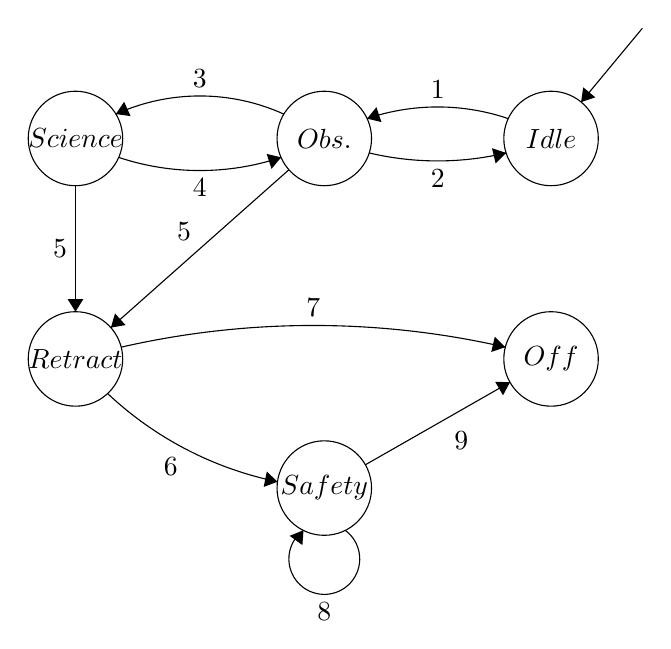
\begin{tikzpicture}[scale=0.2]
\tikzstyle{every node}+=[inner sep=0pt]
\draw [black] (46.2,-13.5) circle (3);
\draw (46.2,-13.5) node {$Idle$};
\draw [black] (31.8,-13.5) circle (3);
\draw (31.8,-13.5) node {$Obs.$};
\draw [black] (16,-13.5) circle (3);
\draw (16,-13.5) node {$Science$};
\draw [black] (16,-27.5) circle (3);
\draw (16,-27.5) node {$Retract$};
\draw [black] (46.2,-27.5) circle (3);
\draw (46.2,-27.5) node {$Off$};
\draw [black] (31.8,-35.7) circle (3);
\draw (31.8,-35.7) node {$Safety$};
\draw [black] (52,-6.5) -- (48.11,-11.19);
\fill [black] (48.11,-11.19) -- (49.01,-10.89) -- (48.24,-10.25);
\draw [black] (34.516,-12.239) arc (108.749:71.251:13.951);
\fill [black] (34.52,-12.24) -- (35.43,-12.46) -- (35.11,-11.51);
\draw (39,-11) node [above] {$1$};
\draw [black] (43.348,-14.419) arc (-76.68931:-103.31069:18.884);
\fill [black] (43.35,-14.42) -- (42.45,-14.12) -- (42.68,-15.09);
\draw (39,-15.43) node [below] {$2$};
\draw [black] (18.564,-11.955) arc (114.4174:65.5826:12.909);
\fill [black] (18.56,-11.95) -- (19.5,-12.08) -- (19.09,-11.17);
\draw (23.9,-10.3) node [above] {$3$};
\draw [black] (29.056,-14.702) arc (-71.60296:-108.39704:16.337);
\fill [black] (29.06,-14.7) -- (28.14,-14.48) -- (28.45,-15.43);
\draw (23.9,-16.04) node [below] {$4$};
\draw [black] (16,-16.5) -- (16,-24.5);
\fill [black] (16,-24.5) -- (16.5,-23.7) -- (15.5,-23.7);
\draw (15.5,-20.5) node [left] {$5$};
\draw [black] (29.55,-15.49) -- (18.25,-25.51);
\fill [black] (18.25,-25.51) -- (19.18,-25.35) -- (18.51,-24.61);
\draw (22.89,-20.01) node [above] {$5$};
\draw [black] (28.83,-35.296) arc (-101.59962:-133.25786:22.283);
\fill [black] (28.83,-35.3) -- (28.15,-34.65) -- (27.95,-35.63);
\draw (22.05,-33.75) node [below] {$6$};
\draw [black] (34.41,-34.22) -- (43.59,-28.98);
\fill [black] (43.59,-28.98) -- (42.65,-28.95) -- (43.15,-29.81);
\draw (40.5,-32.1) node [below] {$9$};
\draw [black] (33.123,-38.38) arc (54:-234:2.25);
\draw (31.8,-42.95) node [below] {$8$};
\fill [black] (30.48,-38.38) -- (29.6,-38.73) -- (30.41,-39.32);
\draw [black] (18.905,-26.751) arc (102.88102:77.11898:54.705);
\fill [black] (43.3,-26.75) -- (42.63,-26.09) -- (42.4,-27.06);
\draw (31.1,-24.87) node [above] {$7$};


\end{tikzpicture}
\end{center}



\begin{center}
Diagram of software states of operation and transition between states [2].

Transitions between states occur as numbered:

\begin{enumerate}
\item{\textbf{Appogee is reached.} The software shall activate when the power line goes to high at 28V. Observation mode shall be 
triggered when the \gls{OBC} turns on. Observation mode will collect a sweep of the payload with the camera. This mode will ensure that the 
camera is operational during the more crticial parts of the mission.}
\item{\textbf{Error: Return to Idle.} If an error is encountered in entering Observation mode, the software shall fallback to Idle 
mode and retry. An error may occur if the payload fails to deploy correctly or if the camera fails to turn on. The system shall send
a signal using the AVR interrupt library if the arm is not fully extended, as the arm is equipped with sensors to determine whether
it is extended or folded. If the camera fails to turn on, the system shall be notified as the telemetry line will be sending empty
data.}
\item{\textbf{Payload Assembly and Camera have been deployed.} The software shall enter Science mode once the payload assembly and arm
 have deployed and the camera has performed an observation sweep. Science mode will consist of the arm touching the sensors in 
 the payload canister, and collecting data via the telemetry line. The whole mode shall be captured with the camera.}
\item{\textbf{Error: Return to Observation} The software shall return to observation mode if any error occurs in Science mode. An error may occur in Science mode if the arm fails to operate correctly and must return to default position. An error may also occur if the camera stops working. The system shall know if the arm fails as a timer can keep track of the time between an arm movement request
and the arm actually completing the movement request. If too much time has elapsed between the request and the movement, the arm may
be stuck. If the telemetry line stops receiving data from the camera, then the camera has stopped working and the system shall be 
notified via an interrupt.}
\item{\textbf{Timer switches to end appogee period.} Once the time period for observation has ended, the timer line will go to low and trigger to Shutdown state. This state can be reached from either Observation or Science mode.}
\item{\textbf{Error: Shutdown not completed successfully.} If an error occurs in the shutdown sequence, the software shall enter Safety mode. An error that could occur is the arm failing to close, the Body failing to retract, or the \gls{OBC} not powering off. All 
these situations except for the \gls{OBC} not powering off are handled through Safety mode.}
\item{\textbf{Retry: Re-attempt to retract the arm.} Attempted to resolve any errors and retry retracting the arm.}
\item{\textbf{Accept: Shutdown correctly} If Shutdown occurs correctly, the arm should be closed, the Arm Assembly Body should be retracted, and the \gls{OBC} should be powered off. The arm will be have sensors to detect whether its closed or not, which can also
be used to know whether it has been retracted into the body. Once the system has determined that this criteria has been met, it
will power off.}
\item{\textbf{Error: Payload is still deployed.} The software shall remain in Safety mode until the payload is either retracted correctly, retracted fully with the arm in the open position, or ejected safely from the rocket. Safety mode shall first try to correctly retract the arm, then retract with the arm open, then repeat attempting ejection until the payload is ejected.}
\item{\textbf{Payload is Shutdown correctly.} If the payload is Shutdown through Safety mode, shutdown can be completed. In Safety mode, the payload was either shut down correctly, retracted fully into the can with the arm open, or the arm was expelled safely from the rocket. The shutdown sequence consists of the arm closing, the Body retracting, and the \gls{OBC} being powered off.}
\end{enumerate}
\end{center}

\subsubsubsection{Target Success Sensors}
\textbf{Author:} Amber Horvath
\label{subsec:tests}
\subsubsubsubsection{Requirement Overview}
The software shall know whether or not the arm succeeded in touching the targets generated, as described in subsection 2.1. The sensors
shall report back whether or not contact was made. This data can be used in post-mortem analysis to determine whether
certain targets were faulty or whether the range of motion on the arm was faulty.
\subsubsubsubsection{Solution Design}
The payload shall be equipped with pre-placed sensors that the arm shall make contact with. The arm shall have generated targets
as described in subsection 2.1. These coordinates shall be stored within the system and used as inputs for the function controlling
the arms' movements, with the target position being where the tip of the arm should be located. The arm shall exert force to touch
the sensor, and the sensor shall go high if contact is made. The sensors high or low signal shall be sent via the telemetry
line and written to our SD card. If the arm gets stuck during this process, it will enter Safety mode, as described in subsection 2.5. The telemetry data shall
later be visualized using Python's UI package, TK. 

\subsubsubsection{Telemetry}
\textbf{Author:} Michael Humphrey
\subsubsubsubsection{Requirement Overview}
The telemetry component shall report via telemetry all error codes and test results.

\subsubsubsubsection{Solution Design}
The telemetry component is responsible for collecting and sending data through the
telemetry ports on the \gls{payload}.

This component shall not be responsible for transmitting data generated from the
temperature sensors.
The temperature sensors will be wired directly to an analog telemetry port,
bypassing the \gls{OBC} altogether.

For each test the software successfully completes (see \hyperref[subsec:tests]{subsection 
\ref*{subsec:tests},  Target Success Sensors}) this component shall output a code
representing the test number to the telemetry port.
There shall be two tests; one for each touch point on the \gls{payload}.
The tests shall be designed as a joint effort between the Hephaestus Structures,
Robotics, Electrical, and Software teams.

The output shall be encoded as a four character \gls{binstring} and transmitted
simultaneously via a four parallel port pins.
The \gls{binstring} shall be transmitted at a rate of no more than 5,000 Hz.
There shall be a delay of no less than .2 milliseconds between transmissions
of codes.
When no code is being actively transmitted, the telemetry shall output a code
of `0000' to the telemetry pins.

In addition to transmitting codes via the telemetry lines, the software shall also
store a log file with timestamps on an onboard SD card.
The log file shall consist of a series of lines of text, consisting of a timestamp
and a description.
The timestamp shall be the number of tenths of milliseconds since the \gls{OBC}
powered on.
The description shall be a sequence of \gls{ASCII} characters of arbitrary length,
and terminated with a carriage return character.

\subsubsubsection{Video Handling}
\textbf{Author:} Michael Humphrey
\subsubsubsubsection{Requirement Overview}
Video footage of the \gls{payload}'s operations shall be recorded and saved to the
SD card.

\subsubsubsubsection{Solution Design}
The Hephaestus Electrical Engineering team shall design the payload such that the 
camera will power on and off at the appropriate times, as well as save footage to
the SD card. 

\subsubsubsection{Data Visualization and Processing}
\textbf{Author:} Michael Humphrey
\subsubsubsubsection{Requirement Overview}
The data visualization and processing component shall provide visualizations
for the collected data.
This component shall be able to show whether the mission success criteria have
been met or not.
If the mission success criteria have not been met, this component shall show how
and why they have not been met.

\subsubsubsubsection{Solution Design}
The component shall have a \gls{gui} written in Tkinter with graphs generated by
\gls{matplotlib}.
The \gls{gui} shall consist of two graphs, a table, and a timeline.
Each graph shall be a \gls{plot} with analog data collected from each of two temperature sensors.
The data from the temperature sensors shall be graphed with respect to time from
\gls{apogee} and actual temperature, if such a value can be determined.
In the absence of a method to reliably determine actual temperature from the raw
sensor data, then the data shall be graphed with respect to the raw value received
from the sensor, with the graph scaled such that the lowest value recorded shall be
the minimum y value, and the highest recorded value recorded shall be the maximum y value.
The user shall be able to scale the graphs to view portions of the data as they see fit.
The table shall consist of the name of each of a series of tests,
the result of that respective test, and the time that test was completed.
A result shall be either ``passed'', ``failed'', or ``not completed''.
A result of ``passed'' shall be colored in green.
A result of ``failed'' shall be colored in red.
A result of ``not completed'' shall be colored in yellow.
If the result of a test is ``not completed'', then the time of completion for that test
may be omitted.
There shall be two total tests.
The tests shall be for if the \gls{payload} can successfully touch each touch point sensor.
The tests shall be designed as a joint effort between the Hephaestus Structures,
Robotics, Electrical, and Software teams.
The timeline shall be a visualization with time on the y axis, with significant events
marked at various positions along the axis, according to when that event happened.


\subsubsection{Conclusion}
This concludes the design of our project. Further questions or concerns can be addressed to the authors of this document.
This document may be subject to changes in the future as more design constraints are found, or designs are found to not work the way

